\documentclass[UTF8]{ctexart}
\usepackage{dirtree}
\usepackage{listings}
\usepackage{xcolor}
\usepackage{graphicx}
\usepackage{enumerate}
\usepackage[a4paper]{geometry} 
\usepackage{amsmath,amsthm,mathtools}
\usepackage{mathtools}
\usepackage{diagbox}
\usepackage{multirow,makecell}
\usepackage{url}
\newcommand{\refe}[1]{Eq.\ref{#1}}
\newtheorem{theory}{Theory}[section]
\newcommand{\reffig}[1]{\,\emph{图\ref{#1}}\,}
\title{Lab3-线程通讯}
\author{张配天-2018202180}
\date{\today}
\geometry{head=1cm,bottom=1cm,left=2cm,right=2cm}

\lstset{
 columns=fixed,       
 numbers=left,                                        % 在左侧显示行号
 numberstyle=\tiny\color{gray},                       % 设定行号格式
 basicstyle=\ttfamily,
 frame=none,                                          % 不显示背景边框
 backgroundcolor=\color[RGB]{245,245,244},            % 设定背景颜色
 keywordstyle=\color[RGB]{40,40,255},                 % 设定关键字颜色
 numberstyle=\footnotesize\color{darkgray},           
 commentstyle=\color{gray}\ttfamily,                % 设置代码注释的格式
 stringstyle=\rmfamily\slshape\color[RGB]{128,0,0},   % 设置字符串格式
 showstringspaces=false,
 breaklines=true,
 language=c++
}

\begin{document}
    \maketitle
    \tableofcontents
    \section{实验目的}
    \begin{itemize}
        \item 加深对线程和多线程概念的理解;
        \item 掌握多线程程序设计的基本方法;
        \item 学习同一进程内线程间交换数据的方法    
    \end{itemize}

    \section{实验思想和方法}
    \begin{itemize}
        \item 自行学习线程间通讯的锁机制
        \item 实践互斥锁、条件变量和信号量
        \item 由于线程和父进程共享资源的特点,使用共享内存而非管道避免二次拷贝和二次读取
        \item 用ascii码来判断输入的是字母还是数字
    \end{itemize}
    
    \section{程序结构及算法}
    \subsection{锁的声明}
    \begin{itemize}
        \item 全局变量char buff\_input[100] = “”,作为共享的资源,存储输入字符串;
        \item 互斥锁mutex\_buff,实现输入和显示线程的互斥;
        \item 条件变量toDisplay,实现输入后显示的同步;
        \item 信号量toProcess,实现输入字符串后处理字符串的同步;
        \item 信号量toNotify,实现处理好字符串后显示信息的同步;
    \end{itemize}
    \subsection{锁的设计}
    \begin{itemize}
        \item 输入和读取不能同时访问临界区资源(即buff\_input),因此使用互斥锁保证先写再读;
        \item 在输入完之后才能进行显示,因此在互斥锁内部使用条件变量实现同步,保证输入完成后再显示;
        \item 由于处理输入的线程和显示线程只有同步关系而非互斥关系,因此使用信号量完成同步(条件变量必须在锁内部使用),保证输入完成后再进行字符串处理;
        \item 字符串处理结束后唤醒显示线程输出信息,因此再次使用信号量完成同步。
    \end{itemize}
    \section{实验结果}
        运行结果如下:
        \begin{figure}[htb]
            \centering
            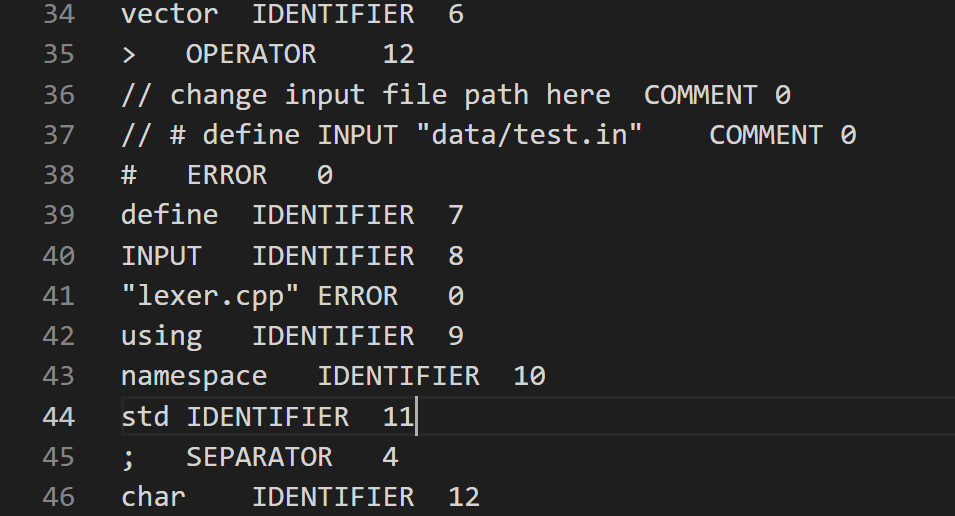
\includegraphics[width=15cm]{resources/result.png}
            \caption{运行结果}
            \label{}
        \end{figure}
        其中letters.txt,numbers.txt的结果如下:
        \begin{figure}[htb]
            \centering
            \includegraphics[width=10cm]{resources/letters.png}
            \caption{letters.txt}
            \label{}
        \end{figure}
        \begin{figure}[htb]
            \centering
            \includegraphics[width=10cm]{resources/numbers.png}
            \caption{numbers.txt}
            \label{}
        \end{figure}
        \section{问题探究}
        \subsection{死锁}
        \begin{itemize}
            \item 如果把pthread\_cond\_wait()放在互斥锁外执行则会引起死锁,因为该函数为了保证即使条件变量得到满足,仍然仅能有1个线程访问临界区,会在运行结束后自动将互斥锁闭合。\par
            \item pthread\_cond\_signal()的位置便比较灵活
        \end{itemize}
        
        \subsection{段错误}
        如果将互斥锁指针参数传为NULL,则会引起段错误

\section{思考}
线程通讯和进程通讯的不同之处在于线程可以访问父进程的资源,使得通讯比进程更为方便。

        \section{源代码}
        \begin{lstlisting}
#include <stdio.h>
#include <stdlib.h>
#include <pthread.h>
#include<string.h>
#include<semaphore.h>


char inputBuff[100] = "";
pthread_mutex_t mutex_buff;
pthread_cond_t toDisplay;//toProcess;
sem_t toProcess,toNotify;//用条件变量的时候必须满足其和output进程的互斥,但是process进程和output进程没有互斥关系
pthread_t tid1,tid2,tid3;

void * KCP_input(){
    pthread_mutex_lock(&mutex_buff);
    printf("请输入数据:");
    scanf("%s",inputBuff);
    //pthread_cond_signal(&toDisplay);

    pthread_mutex_unlock(&mutex_buff);
    //条件变量的signal的位置要求不严格,因为其不涉及开锁再关锁的行为
    pthread_cond_signal(&toDisplay);
    sem_post(&toProcess);
    //pthread_cond_signal(&toProcess);
    return (void*)0;
}
void * DCP_output(){    
    //cond_wait必须放在互斥锁内部,否则由于其机制是收到相应条件变量后会再次把该锁锁上,会造成死锁
    //pthread_cond_wait(&toDisplay,&mutex_buff);
    pthread_mutex_lock(&mutex_buff);
    pthread_cond_wait(&toDisplay,&mutex_buff);
    printf("%s\n",inputBuff);
    pthread_mutex_unlock(&mutex_buff);
    printf("-------processing data--------\n");
    sem_wait(&toNotify);
    printf("Process completed!\n");
    return (void*)0;
}
void * CCP_dispose(){
    sem_wait(&toProcess);
    FILE * fp_num = fopen("numbers.txt","w");
    FILE * fp_let = fopen("letters.txt","w");
    //pthread_mutex_lock(&mutex_buff);
    //pthread_cond_wait(&toProcess,&mutex_buff);
    for(int i = 0;i < strlen(inputBuff);i++){
        int c = (int)inputBuff[i];
        if(c<= 57 && c>=48){
            fputc(inputBuff[i],fp_num);
        }
        else if(c<=122 && c>=65){
            fputc(inputBuff[i],fp_let);
        }
    }
    sem_post(&toNotify);
    //关闭文件
    fclose(fp_let);
    fclose(fp_num);
    return (void*)0;
}

int main(){

    pthread_mutex_init(&mutex_buff,NULL);
    //pthread_cond_init(&toProcess,NULL);
    pthread_cond_init(&toDisplay,NULL);
    sem_init(&toProcess,1,0);//同步
    sem_init(&toNotify,1,0);//同步

    
    //默认先创建的的线程会先执行
    pthread_create(&tid1,NULL,DCP_output,NULL);
    pthread_create(&tid2,NULL,CCP_dispose,NULL);
    pthread_create(&tid3,NULL,KCP_input,NULL);
    
    pthread_join(tid1,NULL);
    pthread_join(tid2,NULL);
    pthread_join(tid3,NULL);
    //等待所有线程完成任务后释放内存
    pthread_cond_destroy(&toDisplay);
    pthread_mutex_destroy(&mutex_buff);
    sem_destroy(&toProcess);
    sem_destroy(&toNotify);
    
    return 0;
}
\end{lstlisting}
\end{document}